\documentclass[13pt, ignorenonframetext]{beamer}
%\documentclass[13pt, handout, notes, gray]{beamer}
%\usepackage{handoutWithNotes}
%\usepackage{pgfpages}
%\pgfpagesuselayout{2 on 1 with notes landscape}[a4paper,border shrink=5mm]

\usetemplatenote{{\footnotesize \begin{quote} \insertnote \end{quote}}}

\usepackage[utf8]{inputenc}
\usepackage{parskip}
\usepackage{url}
\usepackage{listings}
\usetheme{AnnArbor}

\setbeamertemplate{navigation symbols}{}
\institute[PUG@Canberra]{PUG Meetup   \\
Canberra}

\title[Centralised logfile analysis using ELK]{Centralised logfile analysis using Elastic, Logstash and Kibana (ELK)}
\author[Tomas Krajca]{Tomas Krajca \\{\tiny $\langle tomas@repositpower.com \rangle$}}
\date{\today}

\newcommand{\comment}[1]{}

\begin{document}

\begin{frame}[plain]
	\titlepage
\end{frame}
%%%%%%%%%%%%%%%%%%%%%%%%%%%%%%%%%%%%%%%%%%%

%These should provide a summary of (a) your initial problem specification; (b) relevant related work and background sources; (c) the approach you took to solving the problem; and (d) the outcomes of your work.
% 20 mins

\section{Outline}
\frame
{
  \frametitle{Today}
  \begin{enumerate}
  \item Reporting state of (python) programs.
  \item Storing these reports.
  \item Processing/indexing these reports.
  \item Searching/analyzing these reports.
  \item ELK pipelines.
  \item Alerting from these reports.
  \item Lessons learned.
  \item QA.
  \end{enumerate}
}
%%%%%%%%%%%%%%%%%%%%%%%%%%%%%%%%%%%%%%%%%%%

\section{Reporting state of (python) programs}
\AtBeginSection[]{
  \begin{frame}
  \vfill
  \centering
  \begin{beamercolorbox}[sep=8pt,center,shadow=true,rounded=true]{title}
    \usebeamerfont{title}\insertsectionhead\par%
  \end{beamercolorbox}
  \vfill
  \end{frame}
}
\begin{frame}
\frametitle{Why and how?}
\begin{enumerate}
\item example1.py
\item example2.py
\item example3.py
\item example4.py
\item logging.ini
\item https://docs.python.org/2/library/logging.html
\item https://docs.python.org/2/library/logging.config.html
\end{enumerate}
\end{frame}


\section{Storing these reports}
\AtBeginSection[]{
  \begin{frame}
  \vfill
  \centering
  \begin{beamercolorbox}[sep=8pt,center,shadow=true,rounded=true]{title}
    \usebeamerfont{title}\insertsectionhead\par%
  \end{beamercolorbox}
  \vfill
  \end{frame}
}
\begin{frame}[fragile]
\frametitle{Log storage}
\begin{enumerate}
\item File
\item AWS S3
\item Console
\item Rsyslog
\item Heroku
\item ...
\end{enumerate}
\end{frame}


\section{Processing/indexing these reports.}
\AtBeginSection[]{
  \begin{frame}
  \vfill
  \centering
  \begin{beamercolorbox}[sep=8pt,center,shadow=true,rounded=true]{title}
    \usebeamerfont{title}\insertsectionhead\par%
  \end{beamercolorbox}
  \vfill
  \end{frame}
}
\begin{frame}[fragile]
\frametitle{Logs}
\begin{verbatim}
2016-06-02 00:21:06,705 DEBUG connectionpool requests.packages.urllib3.connectionpool PID: 1360  "POST /api/query HTTP/1.1" 200 None
2016-06-02 00:21:06,706 DEBUG worker worker0.55 PID: 1360  Response: [{"metric":"operational.australia.nem.ec.customer.load.P","tags":{"source":"CSIRO-2"},"aggregateTags":[],"dps":{"1401581400":0.09135883301496506,"1401581404":0.33968567848205566,"1401581700":0.11657682061195374,"1401581704":0.3968915045261383,"1401582000": ...
2016-06-02 00:21:06,707 INFO master stsdb_proxy.master PID: 1230  worker0.55 returned 405B for client ^@J
2016-06-02 00:21:07,910 DEBUG master stsdb_proxy.master PID: 1230  Received ['1464826867', '\xdc\xa2\x01@r0\xeb\x0f%\xded\xfa\x94GI\x91\xb8O\xcc6\x00B\x11\x00\xf0N\x00\nwrite\x00\xcc\x04\x00Toperational.australia.nem.ec.meter.voltage\x02\xac\xee\xfb\xf4\n\x9a\x19{C\x02\nphase\x06red\x00\x00bonB\x00\x10inver\x01E,reques']... from client ^@: (testec001)
2016-06-02 00:21:07,910 INFO master stsdb_proxy.master PID: 1230  Proxied 3229B from client ^@: (testec001) to worker0.55
2016-06-02 00:21:07,962 DEBUG worker worker0.55 PID: 1360  POSTing [{"timestamp":1464826774,"metric":"operational.australia.nem.ec.meter.voltage","value":251.1000061035,"tags":{"phase":"red"... to http://dtsdb.repositpower.net/api/put?details
2016-06-02 00:21:07,972 DEBUG connectionpool requests.packages.urllib3.connectionpool PID: 1360  "POST /api/put?details HTTP/1.1" 200 None
2016-06-02 00:21:07,974 INFO master stsdb_proxy.master PID: 1230  worker0.55 returned 12B for client ^@:
2016-06-02 00:21:07,998 DEBUG base zmq.auth PID: 1230  version: '1.0', request_id: '1', domain: u'', address: u'172.16.22.38', identity: '', mechanism: 'CURVE'
2016-06-02 00:21:07,998 DEBUG base zmq.auth PID: 1230  ALLOWED (CURVE) domain=* client_key=6V8>9Y(yBGgg)Uyu}V-s*jKbB3KU9&Ku+T]-Z!(z
2016-06-02 00:21:07,998 DEBUG zmq_ zmq.auth PID: 1230  Authenticated user `c9cce94a1cf344fd8913978528baae21'
2016-06-02 00:21:07,998 DEBUG base zmq.auth PID: 1230  ZAP reply code=200 text=OK
...
\end{verbatim}
\end{frame}


\begin{frame}
\frametitle{Logstash}
\begin{enumerate}
    \item Tool that crunches logs/reports.
    \item Configurable to process any sorts of logs.
    \item Ruby/java.
    \item Collect - Process - Forward events/messages.
    \item Input(s) - Filter(s) - Output(s).
    \item https://www.elastic.co/products/logstash
\end{enumerate}
\end{frame}


\begin{frame}[fragile]
\frametitle{Logstash inputs}
\begin{lstlisting}[basicstyle=\footnotesize]
input {
  file {
    type => "python"
    path => 
      ["/var/log/apps/app.stderr.log"]
    add_field => [ "program", "app" ]
    sincedb_path => 
      "/var/lib/logstash/sincedb"
  }
}
\end{lstlisting}
\end{frame}


\begin{frame}
\frametitle{Logstash filters}
\begin{enumerate}
\item logstash.conf
\item https://github.com/elastic/logstash/blob/v1.4.2/patterns/grok-patterns
\item \$ logstash -v -f ~/logstash.conf
\end{enumerate}
\end{frame}


\begin{frame}[fragile]
\frametitle{Logstash filters}
\begin{lstlisting}[basicstyle=\scriptsize]
{
          "message" => "2016-06-01 12:52:41,129 DEBUG base zmq.auth 
                        PID: 1230  ZAP reply code=200 text=OK",
         "@version" => "1",
       "@timestamp" => "2016-06-01T12:52:41.129Z",
             "host" => "dauvmfes001.repositpower.net",
             "path" => "/var/log/apps/SecureTSDBProxy.stderr.log",
             "type" => "python", 
          "program" => "SecureTSDBProxy",
         "loglevel" => "DEBUG",
           "module" => "base",
           "logger" => "zmq.auth",  
      "received_at" => "2016-06-01T12:52:41.182Z",
    "received_from" => "dauvmfes001",
     "@source_host" => "dauvmfes001",
         "@message" => "ZAP reply code=200 text=OK",
             "tags" => [
        [0] "_parsed"
    ]
}
\end{lstlisting}
\end{frame}


\section{Searching/analyzing these reports}
\AtBeginSection[]{
  \begin{frame}
  \vfill
  \centering
  \begin{beamercolorbox}[sep=8pt,center,shadow=true,rounded=true]{title}
    \usebeamerfont{title}\insertsectionhead\par%
  \end{beamercolorbox}
  \vfill
  \end{frame}
}
\begin{frame}[fragile]
\frametitle{Logstash outputs}
      \begin{columns}[c] % contents are top vertically aligned
     \begin{column}{3.0cm} % each column can also be its own environment
\begin{enumerate}
\item Zabbix
\item Redis
\item Elasticsearch
\item ...
\end{enumerate}
     \end{column}
     \begin{column}{6.0cm} % alternative top-align that's better for graphics
\begin{lstlisting}[basicstyle=\scriptsize]
output {
  if "zabbix" in [tags] {
    zabbix {
      host => "zabbix.repositpower.net"
      port => "10051"
      zabbix_sender => 
        "/usr/bin/zabbix_sender_retry"
    }
  }
  elasticsearch {
    host => "search.repositpower.net"
    protocol => "http"
    flush_size => 1000
    max_retries => 7
  }
}
\end{lstlisting}
     \end{column}
     \end{columns}
\end{frame}


\begin{frame}
\frametitle{Elasticsearch}
\begin{enumerate}
\item NoSQL database.
\item Scalable, robust, powerful.
\item Full-text search server built on Lucene indexes.
\item (JSON) Schema free.
\item HTTP/JSON or TCP API/interface
\item Java
\item Indexes - Databases
\item https://www.elastic.co/
\end{enumerate}
\end{frame}


\begin{frame}
\frametitle{Elasticsearch demo}
\begin{enumerate}
\item Python client libraries. 
\item https://pypi.python.org/pypi/elasticsearch/2.3.0
\item http://search.repositpower.net:9200/
\item http://search.repositpower.net:9200/\_cat/indices?v
\item curl -d '{"loglevel": "INFO", "@message":"Tomas Krajca2"}' http://search.repositpower.net:9200/test/2/\_update
\item http://search.repositpower.net:9200/logstash-2016.06.02/\_search?q=
      @message:"timed out"\&pretty=true
\item \$ curator show indices --all-indices
\end{enumerate}
\end{frame}

\begin{frame}
\frametitle{Kibana}
\begin{enumerate}
\item Data visualization and search for elasticsearch.
\item https://www.elastic.co/products/kibana
\end{enumerate}
\end{frame}


\begin{frame}
\frametitle{Kibana demo}
\begin{enumerate}
\item time\_duration:[3000 TO *] AND http\_request:*
\item bytes\_read:[3000 TO *] AND http\_request:*
\item loglevel:ERROR OR loglevel:WARNING AND @message:timeout AND NOT @message:Unable
\end{enumerate}
\end{frame}


\section{ELK pipelines}
\AtBeginSection[]{
  \begin{frame}
  \vfill
  \centering
  \begin{beamercolorbox}[sep=8pt,center,shadow=true,rounded=true]{title}
    \usebeamerfont{title}\insertsectionhead\par%
  \end{beamercolorbox}
  \vfill
  \end{frame}
}
\begin{frame}
\frametitle{Distributed}
\begin{enumerate}
\item Logstash + Elasticsearch + Kibana
\end{enumerate}
\begin{figure}
\centering
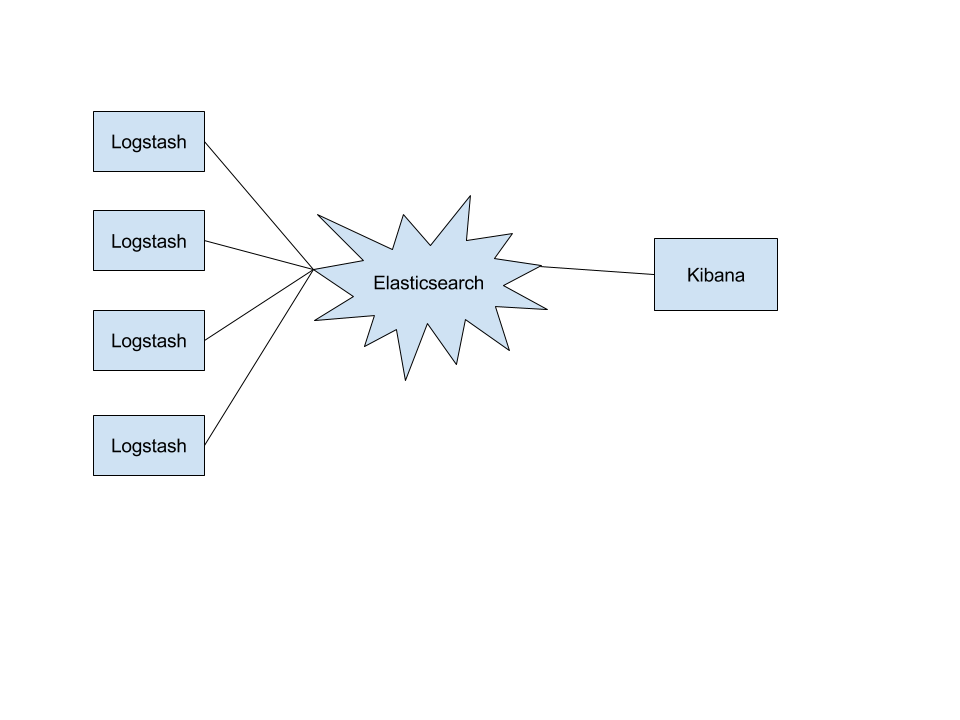
\includegraphics[width=11.0cm]{images/distributed-elk.png}
\end{figure}
\end{frame}

\begin{frame}
\frametitle{Centralized}
\begin{enumerate}
    \item Logstash + Redis + Logstash + Elasticsearch + Kibana
    \item Logstash forwarder/Filebeat + Redis + Logstash + Elasticsearch + Kibana
    \item Rsyslog forwarder + Rsyslog master + Logstash + Elasticsearch + Kibana
\end{enumerate}
\begin{figure}
\centering
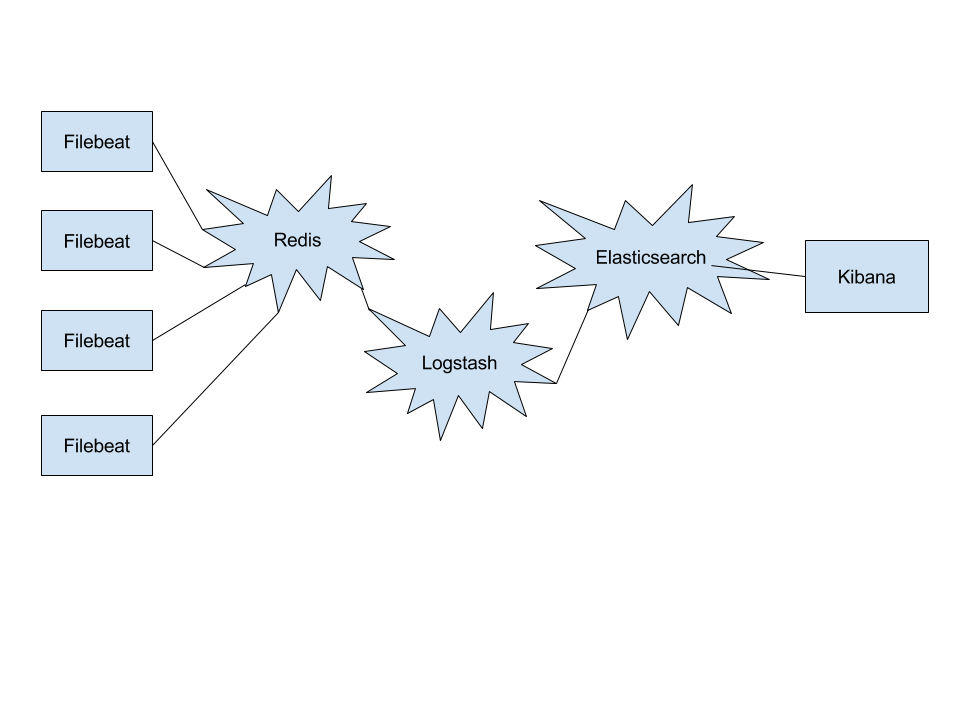
\includegraphics[width=8.5cm]{images/centralized-elk.png}
\end{figure}

\end{frame}


\begin{frame}
\frametitle{Considerations}
\begin{enumerate}
    \item Complexity.
    \item How much logging on each node.
    \item How strict SLAs for each service.
    \item How reliable should it be.
    \item How fast/real-time should it be.
    \item Who does the hard work.
\end{enumerate}
\end{frame}


\section{Alerting from these reports}
\AtBeginSection[]{
  \begin{frame}
  \vfill
  \centering
  \begin{beamercolorbox}[sep=8pt,center,shadow=true,rounded=true]{title}
    \usebeamerfont{title}\insertsectionhead\par%
  \end{beamercolorbox}
  \vfill
  \end{frame}
}
\begin{frame}
\frametitle{Bosun}
\begin{enumerate}
\item Monitoring and alerting system by Stack Exchange.
\item Flexible language to define alerts and notifications.
\item Supports OpenTSDB, Graphite, Elasticsearch, InFlux, ... as backend dbs.
\item https://bosun.org
\end{enumerate}
\end{frame}


\begin{frame}
\frametitle{Bosun demo}
\begin{enumerate}
\item bosun.conf
\item $ max(lsstat("logstash", "backend\_name,server\_name", "program:haproxy,http\_request:.*", "time\_duration", "max", "10s", "5m", "")) > 5000 $
\item lscount("logstash", "@source\_host,program", "loglevel:error", "60s", "3h", "")
\item lscount("logstash", "server\_name,backend\_name", "program:haproxy,http\_request:.*", "1h", "3d", "")
\item Response time alert in rule editor
\item Anomaly-based alerting, alert aggregation.
\end{enumerate}
\end{frame}


\section{Lessons learned}
\AtBeginSection[]{
  \begin{frame}
  \vfill
  \centering
  \begin{beamercolorbox}[sep=8pt,center,shadow=true,rounded=true]{title}
    \usebeamerfont{title}\insertsectionhead\par%
  \end{beamercolorbox}
  \vfill
  \end{frame}
}
\begin{frame}
\frametitle{Tips \& tricks}
\begin{enumerate}
\item Python logging with multiprocessing - avoid files.
\item Advantages of non-blocking/async logging.
\item Don't use multiline logstash input codec.
\item HW resources for logstash and elasticsearch.
\item Event queuing in logstash when elaslticsearch is down.
\item Consensus on meaning of log levels for alerting.
\item Educate staff on using kibana/tools.
\item Never silence python stacktraces.
\item SIGUSR1/SIGUSR2/setupLogging() hooks for dropping logging level, dumping threads and more :).
\item Correlation IDs.
\end{enumerate}
\end{frame}


%%%
\frame[plain]
{
	\begin{center}
	 \textbf{\Large{Questions/discussion}}
\vskip2cm
	\textbf{\Large{Thank you}}
\vskip2cm
	\textit{tomas@repositpower.com}\\
    https://github.com/tkrajca/PUG-ELK
	\end{center}
}

\end{document}
